\section{Method}
\label{section:method}
%In this section, the method used to find an answer to the research questions should be presented. 

%If this report presents results from a literature search, this means providing sufficient information 
%for allowing someone else to repeat the literature search and compare the results. I.e., a search using 
%the phrases a, b, and c, was made in database x, y and z on the date Month Date, Year (e.g., July 31st, 
%2021). The search resulted in x hits. Then, information on how you chose which works to include in this 
%report should be provided. The references should be used for answering your research questions.

%If the work reports on an experiment, this part should provide information about the experimental setup, 
%how the experiment was conducted, how data was collected and analyzed etc. Motivate methodological choices 
%through references. Also an experiment should be presented with sufficient detail such that it can be 
%repeated by someone else.

\subsection{Signal Aqusition}
A setup consisting of a Digilent Analog Discovery studio measurement device, two Myoware muscle sensor 
kits, various weights from none to weights of up to six kilograms and a resistance 
band were used during the signal acquisition. The Myoware sensors were connected to the Analog Discovery 
oscilloscopes, ground and a 3.3 voltage input. Two oscilloscopes were connected to the two Myoware 
sensors, one for the bicep and one for the tricep. The bicep sensor was placed with one end in the 
middle of the biceps brachii while tensed, the other end was placed along the grain of the muscle 
towards the elbow, and the reference was placed between the bicep and triceps on the inside of the arm. 
The triceps sensor was placed with one end in the middle of the long head of the triceps brachii while 
tensed, the other end was placed along the grain of the muscle towards the elbow, and the reference was 
placed either between the bicep and triceps on the inner arm or on the elbow depending on the which would 
be more easily reached. Measurement data was acquired using the Digilent Waveforms program. In Waveforms a 
script was created with javascript code where data was labeled from 0-3 with each state representing a 
different action, 0 = static down, 1 = moving up, 2 = static up, 3 = moving down. Two LED lights showed what 
movement was expected from the user and the data was collected and labeled accordingly. Which test subject, 
which arm, what weight was used and what direction the weight was providing resistance in were all recorded.


\subsection{\acrfull{rnn}}
With the objective of having a reliable method for \acrshort{emg} based continuous motion prediction a \acrshort{rnn} used for the AI model. 
Since the purpose of the project was to end with a working exoskeleton based 
on the RoboRIO system, an embedded solution had to be found. This resulted in two different \acrshort{rnn} 
implementations for the same model:
\begin{itemize}

    \item \textbf{Python implementation:} The first implementation was done using Python and the PyTorch library. 
    This implementation was used to train the model, test its accuracy and extract its parameters.
    
    \item \textbf{LabView implementation:} The second implementation was done using LabView and the RoboRIO system. 
    This implementation was used to import the Python parameters to use the \acrshort{rnn} in a real-time scenario.

\end{itemize}

Before going through with implementing the model, a design was made. The final model was based on the work of Aviles M. et al. \cite{RNNEMG} 
as their \acrfull{lstm} implementation provided promising results both in accuracy and inference time. The model consists 
of four layers:
\begin{itemize}

    \item Input layer

    \item First \acrshort{lstm} layer

    \item Second \acrshort{lstm} layer
    
    \item Output layer

\end{itemize}

The research \cite{RNNEMG} proposed different ranges of values for parameters such as the number of nodes in each one of the \acrshort{lstm} 
layers, the learning rate, and the number of epochs in the training process, which were then optimized by a \acrfull{gwo} 
algorithm for their specific dataset. However, due to hardware restrictions, running such an optimizer was not possible. Instead, 
the parameters were chosen by trial and error where precision and size were taken into account as the model needed to be able to be 
exported to LabView. Figure \ref{fig:rnn_struct} shows the structure of our final model after 
the selection process and table \ref{table:rnn_params} shows the parameters used.

\begin{figure}[h]
    \centering
    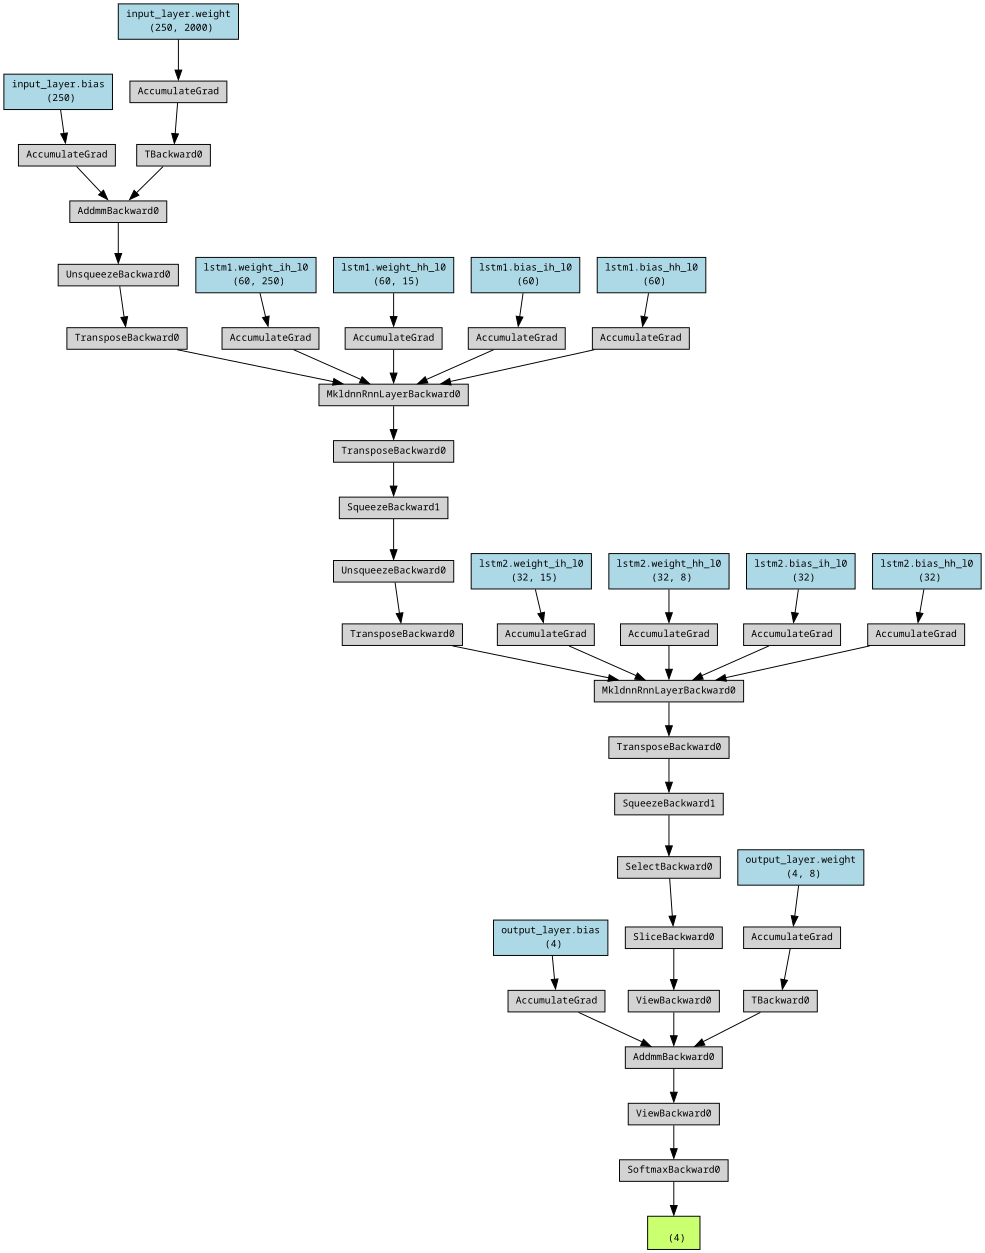
\includegraphics[scale=0.25]{images/rnn_struct.png}
    \caption{Structure of the first \acrshort{rnn} model}
    \label{fig:rnn_struct}
\end{figure}

\begin{table}[h]
    \centering
    \begin{tabular}{|c|c|}
        \hline
        \textbf{Parameter} & \textbf{Value} \\ \hline
        Number of nodes in the input layer & 250 \\ \hline
        Number of nodes in the first \acrshort{lstm} layer & 15 \\ \hline
        Number of nodes in the second \acrshort{lstm} layer & 8 \\ \hline
        Number of output classes & 4 \\ \hline
        Learning rate & 0.00502 \\ \hline
        Number of epochs & 10 \\ \hline
    \end{tabular}
    \caption{Parameters of the first \acrshort{lstm} \acrshort{rnn} model}
    \label{table:rnn_params}
\end{table}

Another model was designed in order to try to solve issues encoutered with the first model. This new model removed the fully connected
input layer and instead of receiving the full windowed data at once, it would receive one input from each sensor in the window at a time.
Figure \ref{fig:rnn_struct2} shows the structure of this new model and the table \ref{table:rnn_params2} shows the parameters used.

\begin{figure}[h]
    \centering
    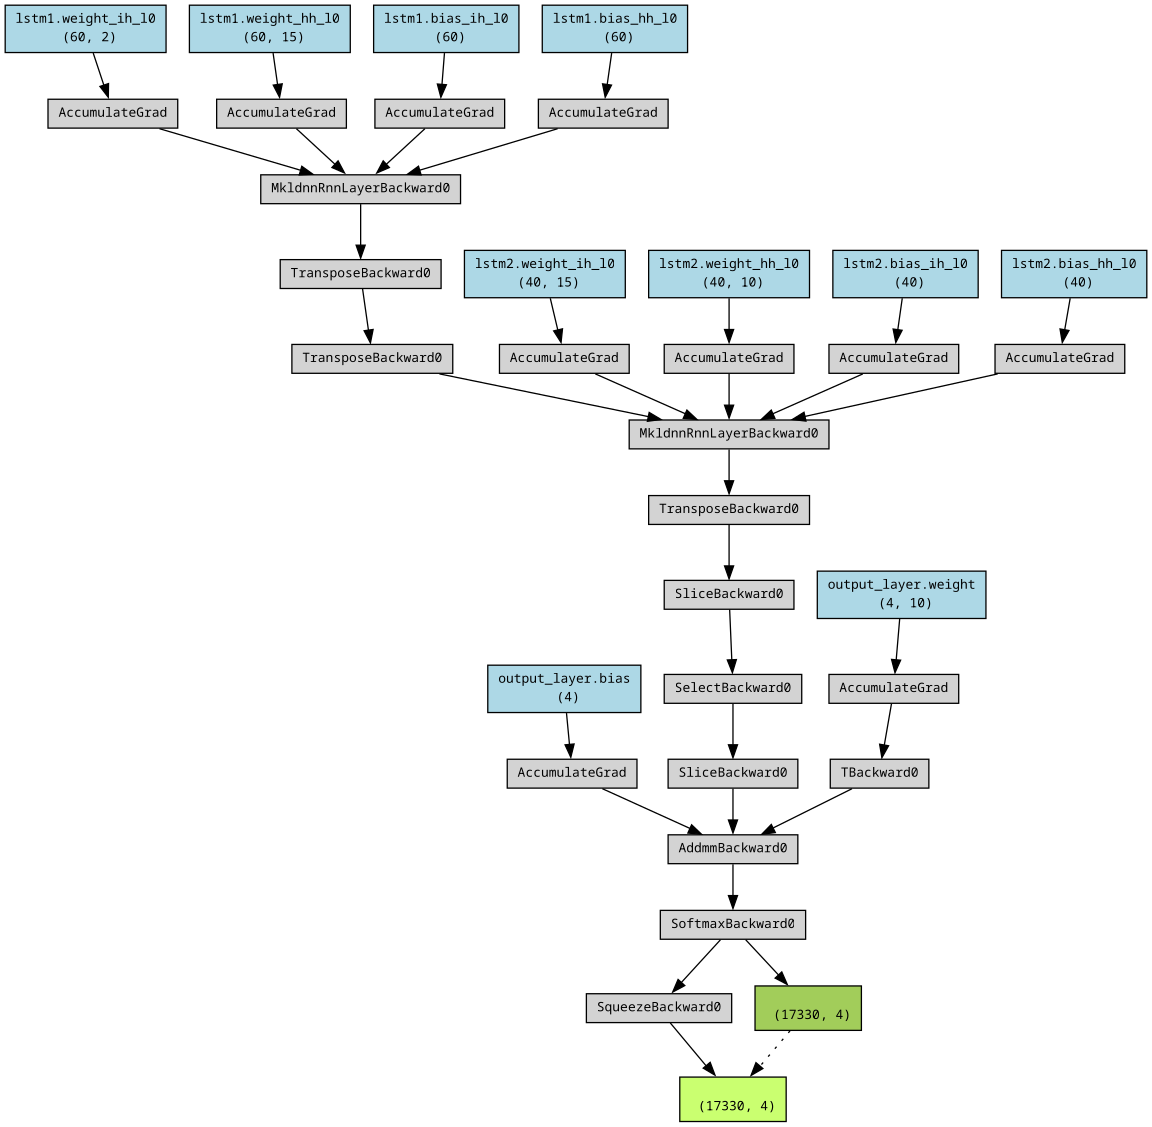
\includegraphics[scale=0.21]{images/rnn_struct_2.png}
    \caption{Structure of the second \acrshort{rnn} model}
    \label{fig:rnn_struct2}
\end{figure}

\begin{table}[h]
    \centering
    \begin{tabular}{|c|c|}
        \hline
        \textbf{Parameter} & \textbf{Value} \\ \hline
        Number of nodes in the first \acrshort{lstm} layer & 15 \\ \hline
        Number of nodes in the second \acrshort{lstm} layer & 8 \\ \hline
        Number of output classes & 4 \\ \hline
        Learning rate & 0.00502 \\ \hline
        Number of epochs & 10 \\ \hline
    \end{tabular}
    \caption{Parameters of the second \acrshort{lstm} \acrshort{rnn} model}
    \label{table:rnn_params2}
\end{table}

\subsection{Python Implementation}
The Python implementation of the \acrshort{rnn} was done using the PyTorch library as it provided facilities 
to create and train the model while using LSTM layers. The model rans over the training set and for every epoch
it was validated to test its accuracy in the validation set and for every class in the validation set. After the model was trained 
and tested, it was saved both in a .pth file and a .xml file to be used in LabView.
Originally, a script using the \acrshort{gwo} algorithm was implemented 
to optimize the parameters of the model, however, due to the limitations mentioned before, this script was not 
used and instead, a different script with a manual parameter selection was used.
\\
[NOTE: This is results:]This implementation was deemed unsatisfactory as the model achieved a precision of 25\% on the validation set no matter the
learning rate or number of epochs used. Additionally, the results consisted of the model only giving one single class as the output
and therefore having a 100\% accuracy on that specific class and a 0\% accuracy on the rest of the classes. 
[NOTE: This is perhaps conclusion?]This led to a stage of debugging the implementation of the model and without successful results, the decision to reimplement 
a model with a slightly different structure was made.
\\
[NOTE: Rewrite into the first results]The new model removed the fully connected input layer and instead of receiving windowed data, the model would receive one input
from each sensor at a time from the windowed data. This new model was trained and tested with the same data as the previous model 
and achieved the same results as the previous model.
\\
[NOTE: This is Conclusion]After inspecting both model implementations and the data used to train and test them, it was concluded that the problem behind the accuracy
of the models might be the data itself. The data files were shuffled before being fed into the model to avoid learning on the test subject
itself, however, the data was not preprocessed in any other way aside from windowing. The data from each file was fed into the model in the 
same order as it was collected, which followed a consistent class order. This consistent class order might have led the model's gradient to 
get stuck in a local minimum, which would explain the 25\% accuracy on the validation set.

\subsection{Labview Implementation}
The LabView implementation was multifaceted, with three distinct parts. The first is the preprocessing, done on a separate machine to process the .xml files into properly set up .bin files able
to be read by the embedded system. The second is data acquisition done on the \acrfull{FPGA} which opens two ports and reads the voltage continuously. The third one is the Real Time system which
initializes all connections, and loads settings and weights. It then runs a loop of data gathering from the \acrshort{FPGA} then running it through the RNN which output is interpreted into a single 
value to be sent through the CAN bus to a motor controller. If the loop is interrupted it follows a termination of all the connections.